%%%%%%%%%%%%%%%%%%%%%%%%%%%%%%%%%%%%%%%%%%%%%%%%%%%%%%%%%%%%%%%%%%%%%%%%%%%%%%%%
% experiment.tex: Chapter describing the experiment
%%%%%%%%%%%%%%%%%%%%%%%%%%%%%%%%%%%%%%%%%%%%%%%%%%%%%%%%%%%%%%%%%%%%%%%%%%%%%%%%
\chapter{Light Dark Matter eXperiment}
\label{chapter:ldmx:experiment}

\ac{ldmx} is a proposed fixed-target experiment aiming to definitively explore
the light dark matter phase space. Even as a proposed experiment, it has a detailed
plan for construction, a beam already in construction, and well established connections
with current technologies used within \ac{hep}. While \ac{ldmx} is not yet built,
it has a well formulated simulation infrastructure that can realistically model
how the detector design responds to various types of interactions happening within it.

\section{The Beam Line}
\todo[Correctness]{Confirm correctness of this section}
\ac{ldmx} is situated at the end of the Linear Accelerator (Linac) at SLAC National Accelerator
Laboratory. The SLAC Linac can provide high energy, high rate, and low intensity electron beams for
the various experiments it hosts. Specifically, the Linac Coherent Light Source (LCLS) is
used to guide the beam (of a certain energy) towards the experimental hall - the upgraded
phase of LCLS (LCLS II \cite{lcls-ii}) is currently under construction and is what will
be used for running with \ac{ldmx}.

The experiment is hosted in End Station A (ESA) at SLAC which requires an additional upgrade to the
Linac in order to recieve its beam. LESA (Linac to ESA) \cite{lesa-design} is also currently being
constructed and will be ready for test beam in early 2025. Part of the infrastructure that
transfers the beam to ESA (Sector 30 Transfer Line -- S30XL) is already constructed and LDMX
components are expected to participate in a test beam run in summer 2024.

\section{Detector Design}
LDMX is a missing momentum experiment and its design is focused on measuring \emph{both} the
incoming and outgoing momenta of charged particles interacting with a thin target such that
any momentum given to undetectable (dark) particles can be precisely determined. This design has
led to four subsystems each with specialized roles.\footnote{These subsystems also take on
additional roles when the full breadth of the \ac{ldmx} physics program is taken into account.
This description just focuses on the \ac{dm} search.}
\begin{enumerate}
  \item \textbf{Trigger Scintillator} Count the number of electrons incident on the target in time to make a trigger decision (more on what a ``trigger'' is below).
  \item \textbf{Tracker} Measure charged particle momenta both before (``Tagger'') and after (``Recoil'') the target.
  \item \textbf{Electromagnetic Calorimeter} (\ac{ecal}) Measure the total energy of electrons, positrons, and photons.
  \item \textbf{Hadronic Calorimeter} (\acs{hcal}) Veto additional particles difficult for other subsystems to measured (muons, pions, hadrons,...).
\end{enumerate}
\cref{fig:ldmx-det} displays these subsystems in a diagram along with a representation of
a dark brem interaction occurrring within the target. \cref{fig:ldmx-render} shows a rendering
of the detector design.

In many \ac{hep} experiments, a ``trigger'' system is necessary in order to filter data defined to
be interesting by the experiment from the wealth of uninteresting (or normal) data that is expected
to be collected at a much higher rate. These trigger systems are the first filter that any data goes
through and are designed to help the experiment obtain a statistically large data sample without
collecting an overwhelming amount of data.
The Trigger Scintillator (yellow-orange in \cref{fig:ldmx-det}) is designed to help inform the trigger
decision by counting the number of electrons present within the detector. It is made of layers of vertically
segmented bars of plastic scintillator. These layers are arranged in pairs where the layers within
each pair are offset from one another to cover any gaps between the bars. These bars are readout in
time to be used within a trigger decision combined with information from the \ac{ecal} and \ac{hcal}.

The Tracker (purple in \cref{fig:ldmx-det}) is a thin silicon strip detector modeled after the
\ac{hps} tracker. These silicon strips are also arranged in layer pairs where one layer is angled
slightly askew relative to the other in the pair to enable reconstruction of three dimensional hit
locations. The part of the tracker upstream of the target (to the left in \cref{fig:ldmx-det}) is
named the ``tagger'' since its purpose is to measure the incident electrons' momenta, rejecting
electrons' with momentum below $30\%$ of the expected beam momentum. The tagger is situated within
the bulk of the magnetic field enabling highly precise measurement of this incident momentum. The
other part of the tracker located downstream of the target (to the right in \cref{fig:ldmx-det}) is
named the ``recoil'' tracker since its job is to measure the momenta of all charged particles
recoiling from interactions within the target. While it is not located within the magnet volume, it
is still situated within the fringe field, allowing functional momentum resolution.

The \ac{hcal} (green in \cref{fig:ldmx-det}) is a sampling calorimeter made up of alternating
layers of steel absorber and plastic scintillator bars. The \ac{hcal} is further subdivided into
the ``side'' \ac{hcal} which is situated around the \ac{ecal} and the ``back'' \ac{hcal}
downstream of the \ac{ecal}. The back \ac{hcal} has the orientation of the scintillator bars
alternate between vertical and horizontal so that clusters and tracks can have three-dimensional
coordinates more preceisely identified.

The \ac{ecal} (blue in \cref{fig:ldmx-det}), as a primary volume of interest within the analysis
discussed here, is given its own diagram \cref{fig:ldmx-ecal}. The \ac{ecal} is also a sampling
calorimeter; however, it uses a different absorber material and a different sensing mechanism to
more precisely measure the energy of electrons, positrons, and photons. The calorimeter is constructed
out of seventeen layers each consisting of tungsten absorber, service materials, and sensitive silicon
sensors. Each of the layers of the detector has two sub-layers of sensitive silicon sensors and each
of these sub-layers are built up out of the hexagonal High-Density boards designed for the CMS
HGCAL upgrade\todo[citation]{CMS HGCAL Citation needed}. These hexagons are arranged in a ``flower''
providing excellent transverse resolution of shower location and shower shape. The layers are built
and arranged in order to space the sensitive silicon sub-layers to give good longitudinal resolution
of showers as well. In total, the designed \ac{ecal} has more than one hundred thousand channels that
can each individually detect particles depositing energies from $\approx 0.1$ MeV up to $\gtrapprox 1$ GeV\todo[confirm]{Confirm extimate of maximum single-hit energy}.
This high granularity calorimeter gives \ac{ldmx} excellent discrimination power
since it can measure the amplitude and location of several incident particles\todo[evidence]{provide
evidence for this precision claim}.
Due to its high performance, the \ac{ecal} is a primary tool for
both designing a trigger decision (with the aid of the Trigger Scintillator's electron count) as well
as downstream analysis separating \ac{sm} background processes from potential \ac{dm} signal.

\begin{figure}
  \centering
  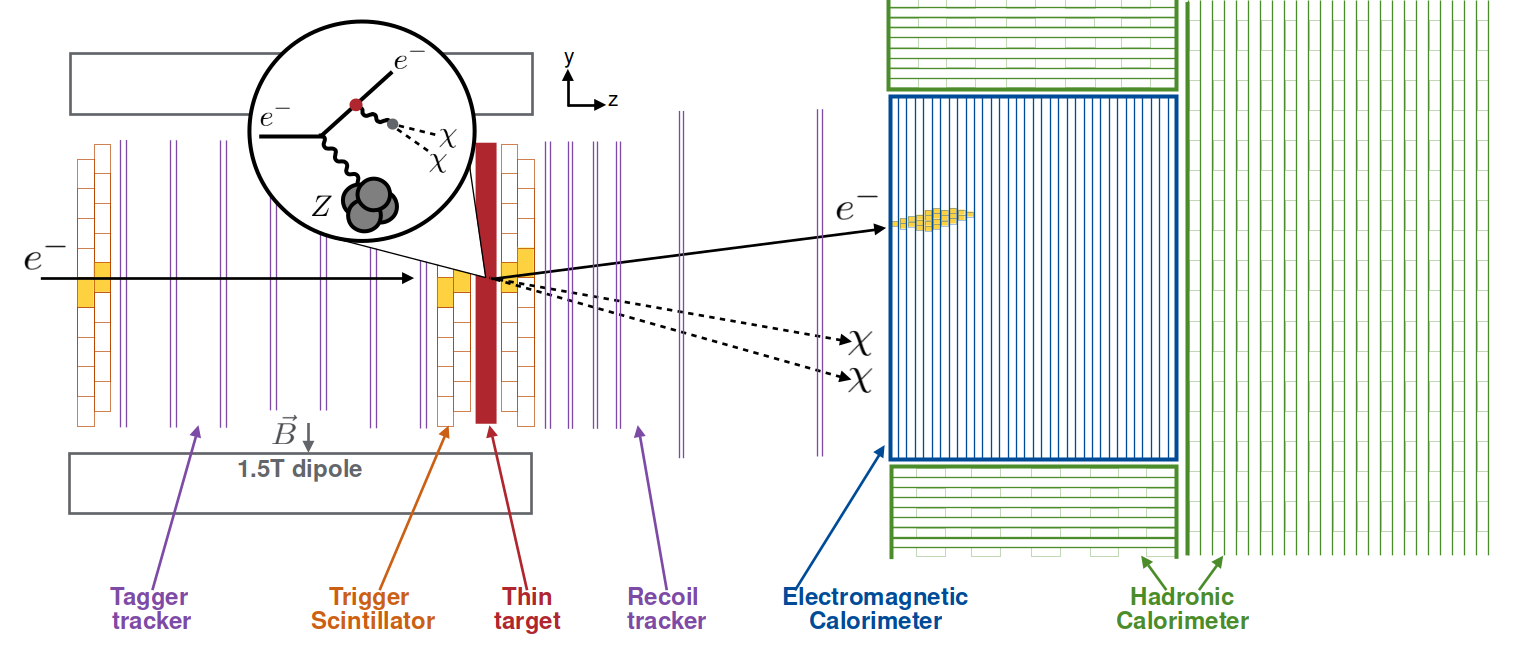
\includegraphics[width=0.9\textwidth]{figures/ldmx/experiment/detector.png}
  \caption{
    Diagram of LDMX detector apparatus with a representation of a signal event where
    a dark brem occurs within the target. Diagram is not to scale. Credit to Christian Herwig
    for original development of diagram.
  }
  \label{fig:ldmx-det}
\end{figure}

\begin{figure}
  \centering
  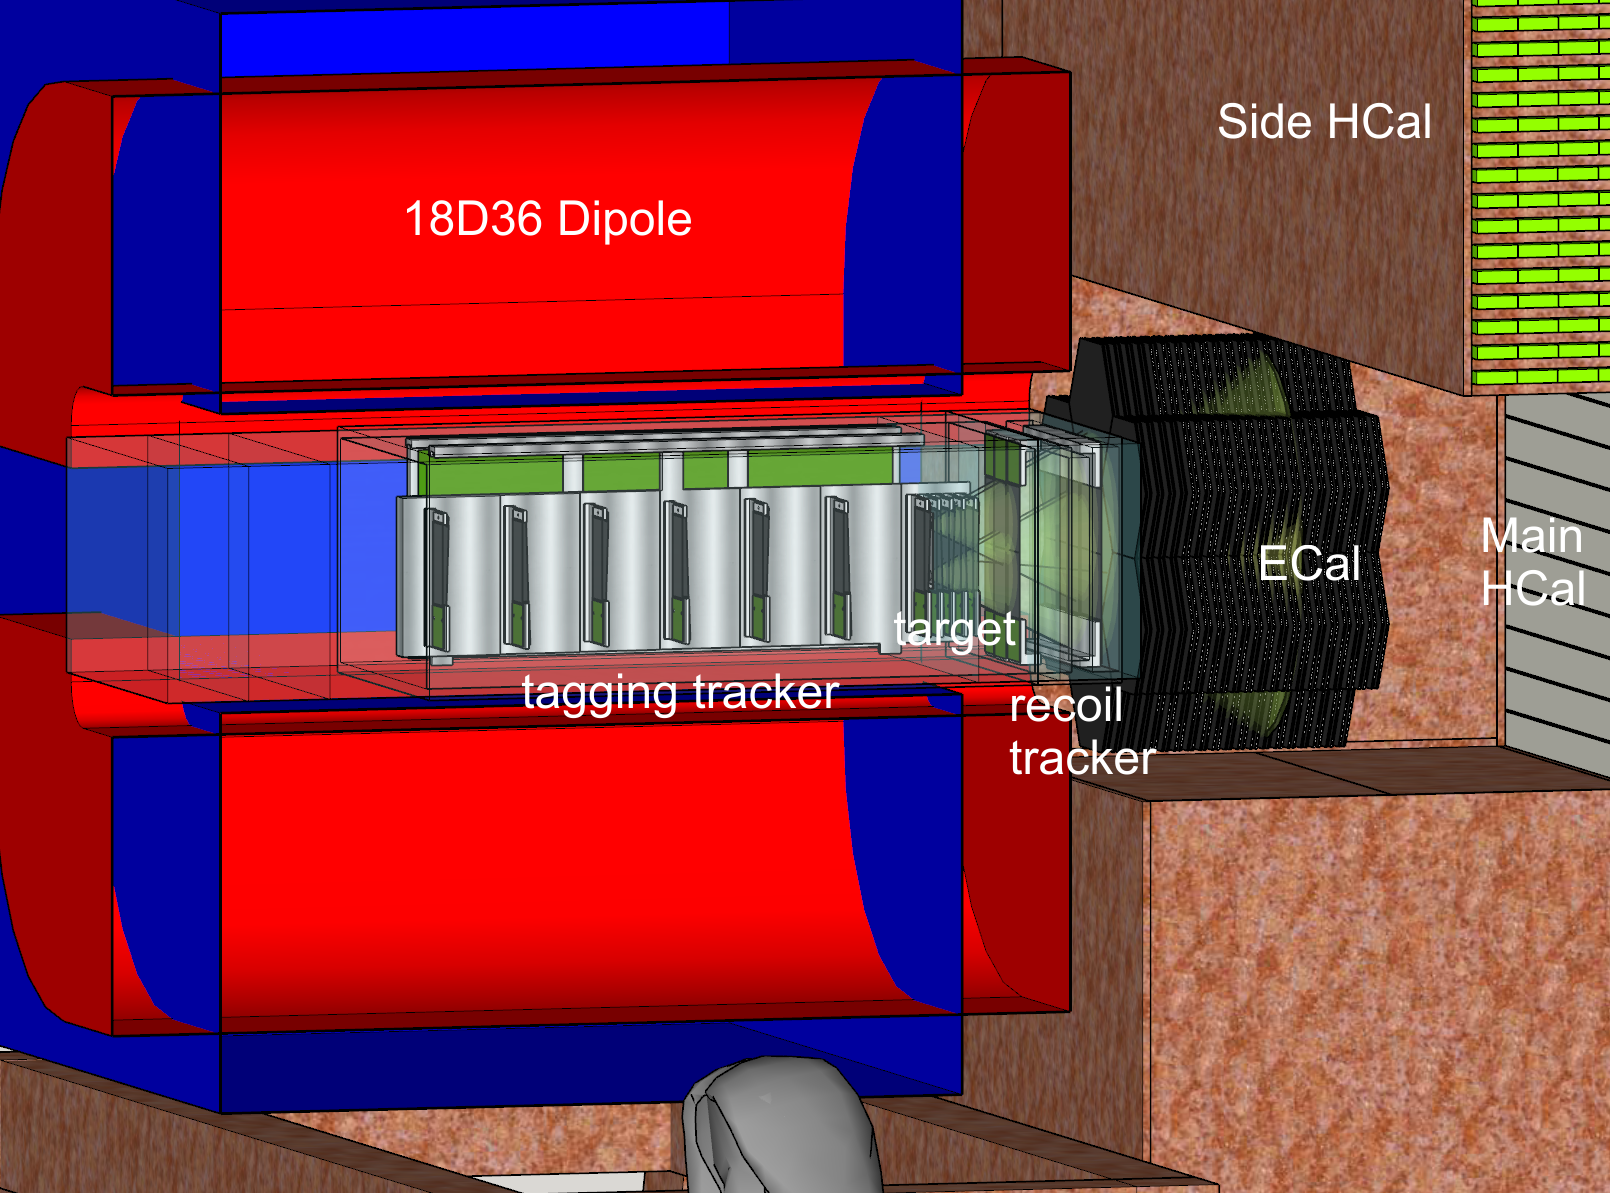
\includegraphics[width=0.9\textwidth]{figures/ldmx/experiment/LDMX_FOA_CLOSE.PNG}
  \caption{
    Rendering of LDMX detector apparatus focusing on tracker, target, and ECal.
    The magnet would fully encompass the tracker, target and trigger scintillator.
  }
  \label{fig:ldmx-render}
\end{figure}

\begin{figure}
  \centering
  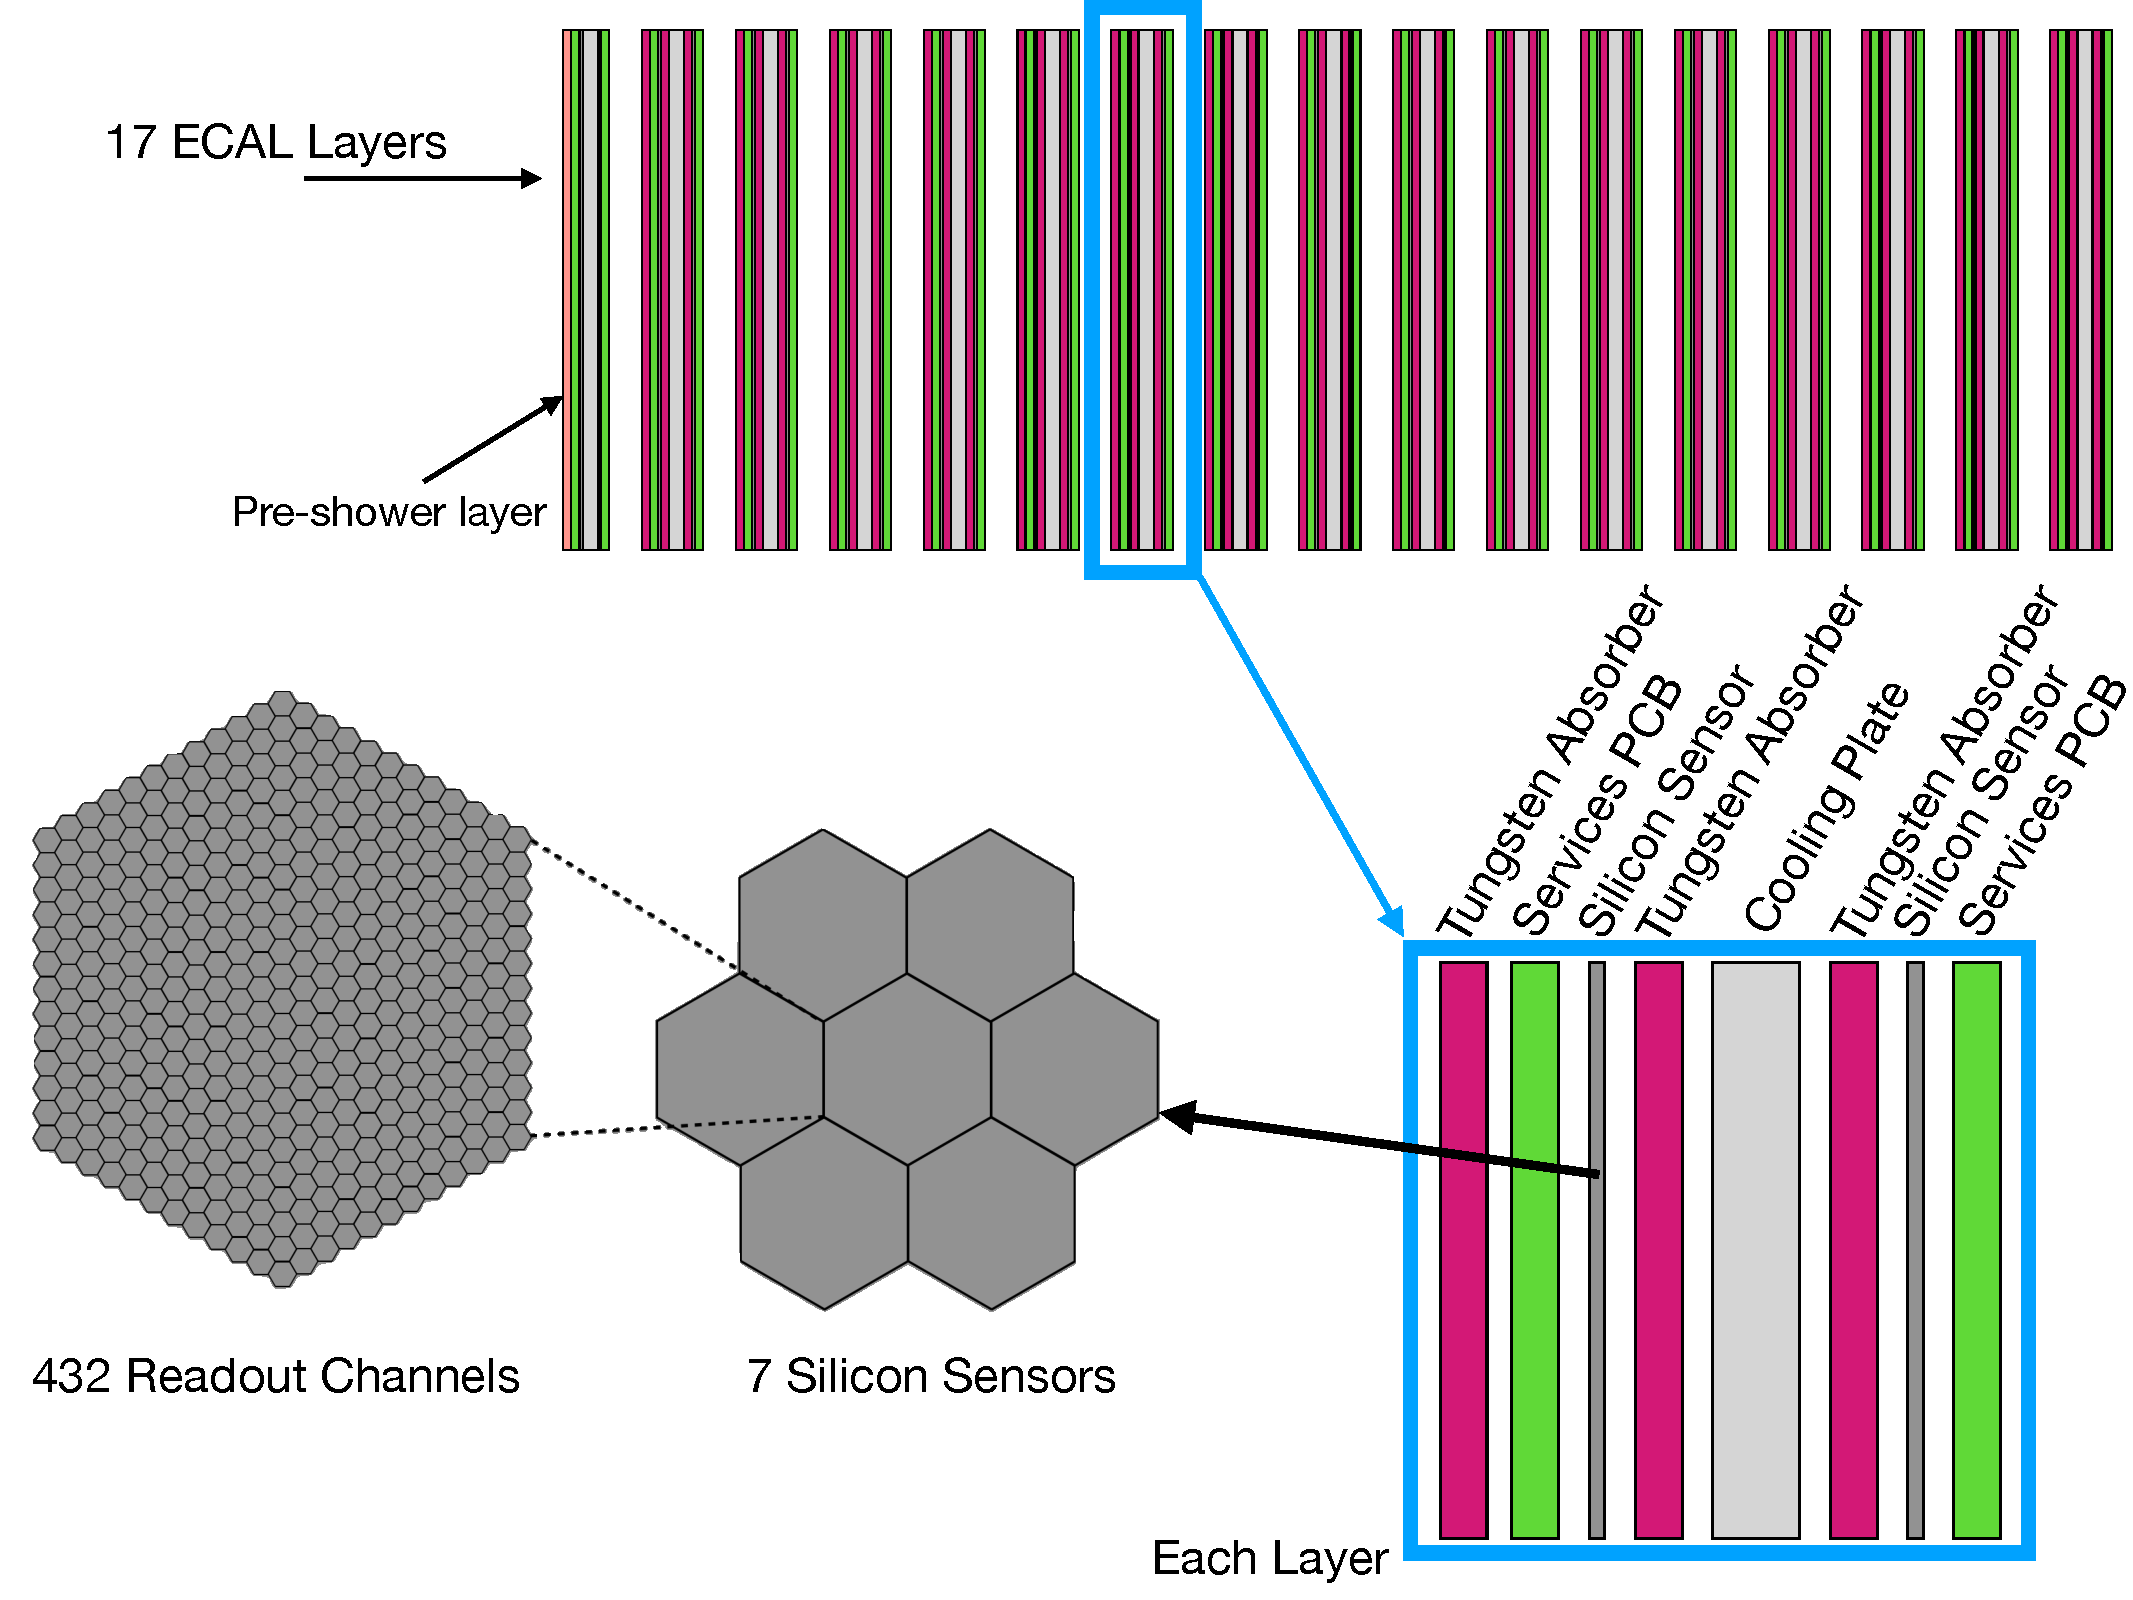
\includegraphics[width=0.9\textwidth]{figures/ldmx/experiment/ecal.pdf}
  \caption{
    Diagram of LDMX \ac{ecal} construction showing the longitudinal segmentation
    (top and bottom right) and the transverse segmentation (bottom left).
    Credit to Joe Muse.
  }
  \label{fig:ldmx-ecal}
\end{figure}

\section{Missing Momentum DM Search}
All of these subsystems can collaborate to help \ac{ldmx} reject known \ac{sm} backgrounds
down to $\sim 10^{-16}$ fraction of all incoming electrons. \cref{fig:ldmx-bkgd-staircase}
displays how the various subsystems veto listed by their relative rate.
With the \ac{ecal}'s excellent energy resolution, it is able to veto the first several
orders of magnitude in basic energy fluctuations including simple interactions in the
target like bremsstrahlung or trident production of an electron-positron pair.
The \ac{ecal}'s capability in this regard has led to the design of the primary
trigger mechanism for \ac{ldmx}: less than $30\%$ of the beam energy observed in the
first twenty senstive silicon layers.

Entering the pink region in \cref{fig:ldmx-bkgd-staircase} is where the background processes
become rarer and more complicated. One of the first ways to partition these backgrounds is
whether charged secondary particles are produced within the target. These ``prompt'' backgrounds
help define the recoil tracker's design and are thus left to be caught by it. More frequently,
a photon is produced within the target (which is not observable by the tracker) and then undergoes
complicated photon-nuclear interactions within the \ac{ecal} producing particles that are difficult
for the \ac{ecal} itself to observe. The \ac{hcal} is able to detect the presence of these hadrons
and muons, acting as a ``pure'' veto in the sense that the signal process should not create
significant activity within it.

\begin{figure}
  \centering
  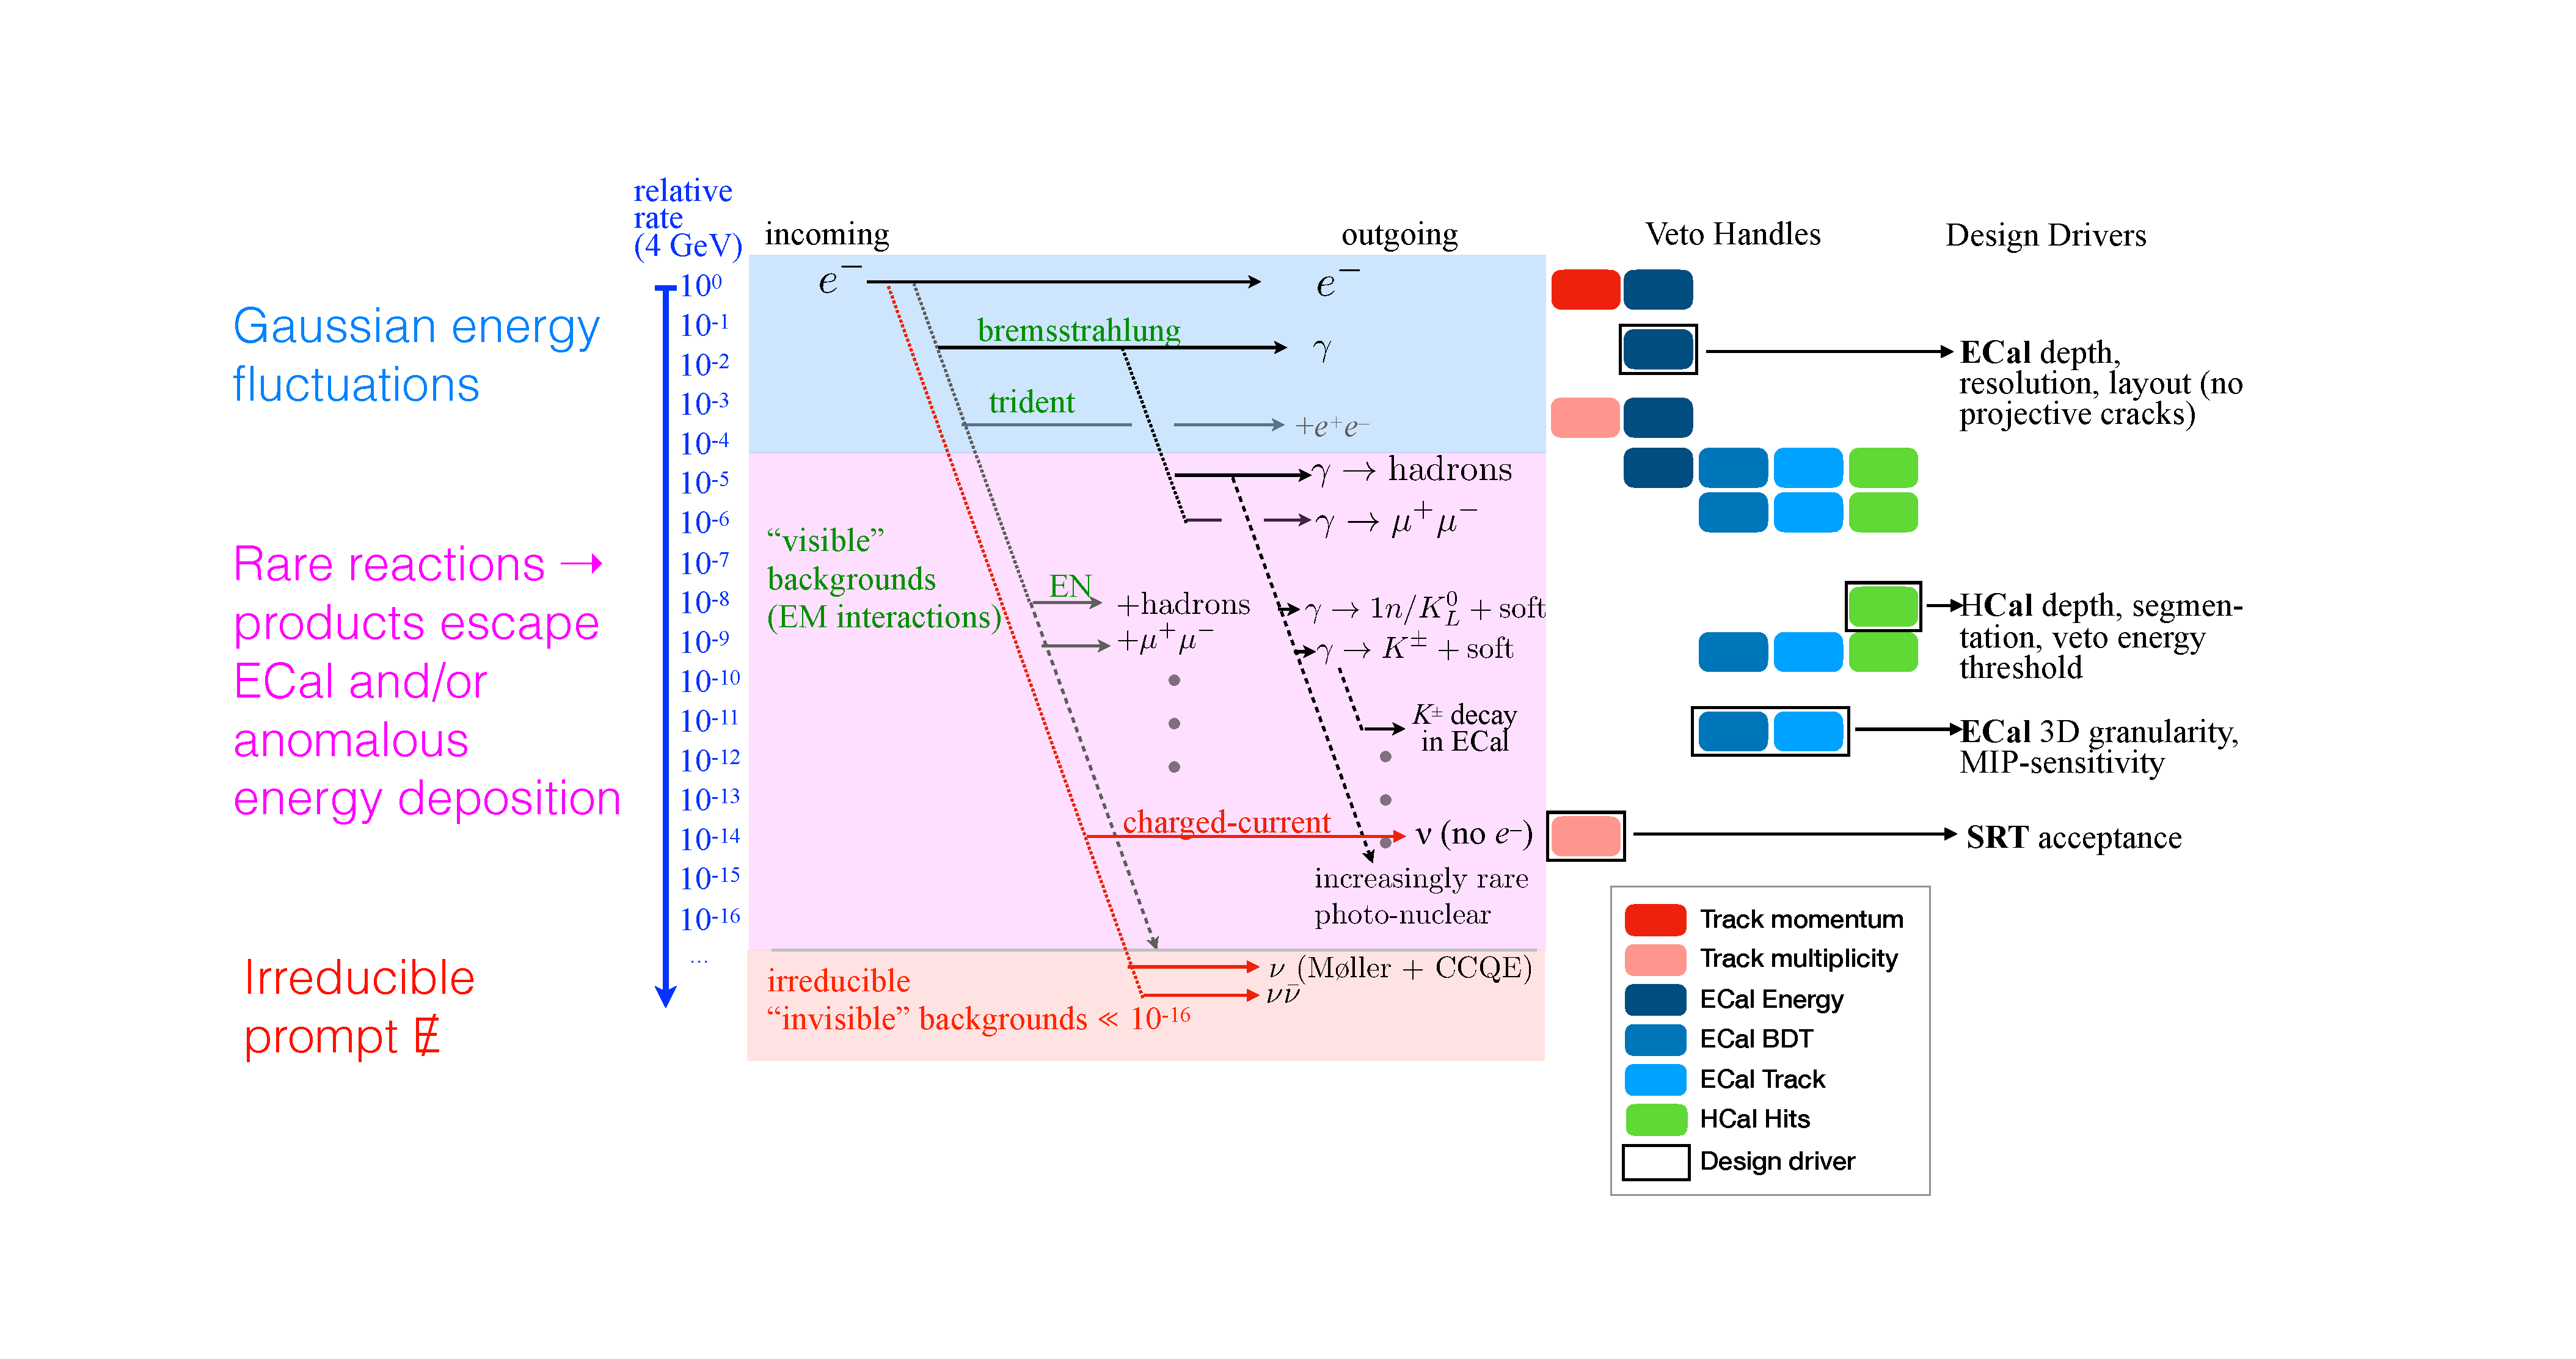
\includegraphics[width=\textwidth]{figures/ldmx/experiment/reaction_staircase_with_designDrivers.pdf}
  \caption{
    Diagram showing relative rates of background processes within LDMX along with
    how they motivate various aspects of the design. $\slash{E}$ stands for ``missing''
    energy or energy that is ``lost'' to neutrinos that are extremely unlikely to be
    detectable within LDMX.
  }
  \label{fig:ldmx-bkgd-staircase}
\end{figure}

Detailed study of the missing momentum search strategy\cite{ldmx-whitepaper,ldmx-photon-reject-2020,ldmx-8gev-2023} show that \ac{ldmx} can reject all simulated backgrounds to a relative rate of $\sim 10^{-14}$\todo[detail]{do we want to report on the detail EoT of the MM analysis?}.
This performance is accomplished through the basic design drivers outlined above and in \cref{fig:ldmx-bkgd-staircase}, but also through the additional granularity of the \ac{ecal} enabling
the use of a \ac{bdt} to distinguish between background and signal events using features of the
showers within the \ac{ecal}.

\section{Missing Energy DM Search}
One of the primary strengths of the LDMX detector design is its ability to use the tagging
and recoil tracker system to reject a large number of background events by separating a nominal
beam with non-standard energy loss from a nominal beam with standard energy loss or even low-energy
beam. Moreover, the tagging and recoil tracker system gives LDMX the potential to further suppress
backgrounds or potentially study DM properties by studying the transverse momenta of electrons
recoiling from dark-bremsstrahlung candidate events.

While this design is optimal for a large number of \ac{eot}, the strategy has some limitations for a low
\ac{eot} data run. To limit multiple scattering which ruins momentum measurements, the baseline detector
configuration requires a thin ($\approx 0.1 \,\mathrm{X}_0$) target. In the early stages of
LDMX, when the total \ac{eot} will be lower, a different analysis strategy and detector configuration
may be optimal to probe the largest amount of the $y$--$m_\chi$ phase space.\todo[introduce]{Provide MM search reach to help give conext to y and mchi.} The alternative
strategy would ignore the dedicated target inside the tracker volume and instead use the \ac{ecal} as an
active target. Using the \ac{eat} for this early-running phase increases the potential
number of dark-bremsstrahlung events and, as long as backgrounds can be suppressed relative to
signal, allows a stronger search capability for a fixed \ac{eot}.

An initial study of the \ac{eat} analysis channel is the primary focus of \cref{part:ldmx} of this thesis. Comparing various signal hypotheses against the pesky photon-nuclear and electron-nuclear background (here called ``Enriched Nuclear") shows that various simple cuts on acitivity in the
\ac{ecal} and \ac{hcal} are able to eliminate necessary amounts of background to achieve significant
and world-leading reach.

%%%%%%%%%%%%%%%%%%%%%%%%%%%%%%%%%%%%%%%%%%%%%%%%%%%%%%%%%%%%%%%%%%%%%%%%%%%%%%%%
